\documentclass[LPSC_Labo03_SDeriaz]{subfiles}


\begin{document}
\section{Simulations}
Les simulations ont été réalisées sur l'itérateur et le loop. Une fois que ces deux blocs ont été vérifiées, la réalisation en pipeline n'as pas été difficile et n'as pas nécessité de testbench.
\subsection{Testbench de l'itérateur}
Une centaine de stimulis sont calculés dans une simulation Python en choisissant des points de départ au hasard dans le plan complexe considéré. Ils sont ensuite stockés dans un fichier texte puis lu par le testbench VHDL, cette approche est très flexible et permet de régénérer rapidement un testbench. Le testbench a permis de trouver beaucoup d'erreurs liées à l'ordre des opérations (nombre d'itération faux de 1 par exemple). Après correction des erreurs de VHDL il a également fallu corriger les arrondis de nombres à virgule fixe dans Python (voir fonction \verb!resize! dans \verb!mandelbrot_functions.py! qui corrige des arrondis effectués par le package). Le testbench final ne montre aucune erreur
\begin{figure}[H]
\centering
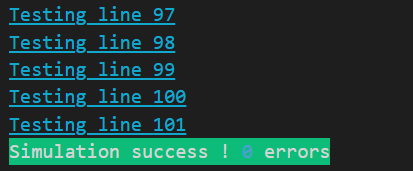
\includegraphics[width=5cm]{testbench_iteration.png}
\caption{Résultat du testbench de l'itérateur}
\label{fig_testbench_iteration}
\end{figure}
En plus du système de lecture de fichiers texte par le banc de test, un système de log avec couleur a été implémenté ce qui permet de générer un fichier compatible avec le standard de couleurs ANSI. Une fois le fichier ouvert dans un terminal Linux ou avec une extension appropriée sur VS Code, il est possible d'observer le log en couleur (voir figure \ref{fig_testbench_iteration})
\subsection{Testbench du loop}
Comme pour le testbench de l'itérateur, un fichier content les stimulis a été généré avec Python. Le testbench a également montré des erreurs de timing (évaluation d'un signal avant ou après sa vraie valeur) mais une fois les erreurs corrigées le testbench ne montre aucune erreur.
\begin{figure}[H]
\centering
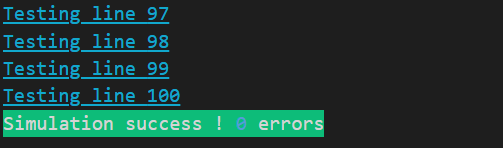
\includegraphics[width=5cm]{testbench_loop.png}
\caption{Résultat du testbench du loop}
\end{figure}







\end{document}